\chapter{\rbscope 的生成}
\label{chap:impl}

本章将详细讨论\dryrun 实现中使用到的\rbscope 生成的一些技术,这部分主要是\dryrun 的第一部分,主要是通过静态分析的方法对给定程序进行无关语句削减。

由于\dryrun 是在LLVM的中间表达形式上实现的转化(LLVM的中间表达形式的特点参见\autoref{chap:IR}),故如无特别说明,下文涉及到的程序的转化都是在LLVM的IR上完成的;由于LLVM的中间形式较为底层并且不易理解,后文采用与之等价的C语言代码来表述。

\section{生成\rbscope 的流程 }
\label{sec:rb_gen}
生成\rbscope 时的流程依赖图如\autoref{fig:rb-gen}所示,其中图中的实线箭头表示流程间的直接依赖关系,虚线箭头表明该依赖关系是可选的;加粗边框的椭圆是可作为最终结果的流程。从图中可以看出,对某一编译单元的分析是精确的指向分析的。
\begin{itemize}
\item 在指向分析的基础上,构建调用图信息。
\item 由于 \autoref{sec:complex} 提及的原因,复杂的关注点可能需要调用图信息来得到其\prog\ps 信息。
\item 在给定指向分析和调用图信息及关注点配置的前提下,削减程序中未被调用的函数。
\item 基于未调用函数削减、关注点配置及调用图完成可达性分析并基于此对程序进行削减。
\item 依赖指向分析、未调用函数削减、关注点配置及调用图信息,进行过程间程序切片;这一过程可以在可达性的削减上进行,也可以在未调用函数削减的基础上进行。
\end{itemize}
上述过程中每一次程序的转化都需要重新建立过程间的分析。

\begin{figure}[t]
\begin{center}
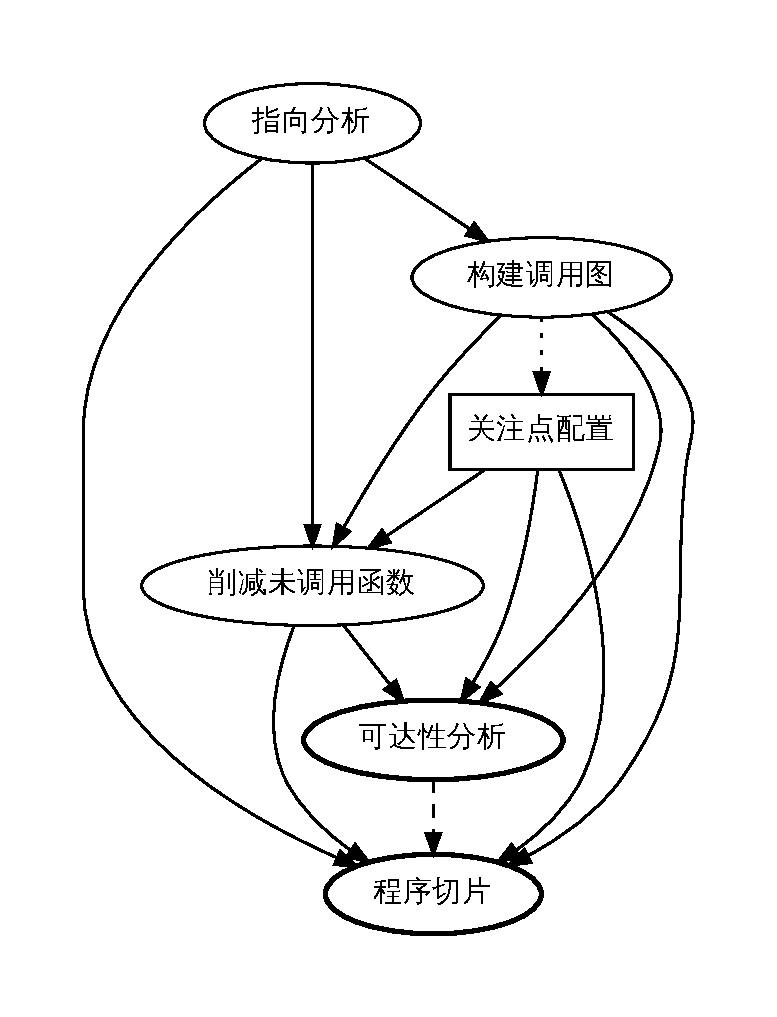
\includegraphics[width=.6\textwidth]{fig/rb_gen.pdf}
\vspace{-24pt}
\bicaption[fig:rb-gen]{生成\rbscope 的流程图}{生成\rbscope 的流程图}{Fig}{Flowchart of \rbscope{} Generation}
\end{center}
\end{figure}

需要说明的是,出于符号执行的需要,通过程序削减生成\rbscope 的过程需遵循下面的基本原则:
\begin{enumerate}
\item 保留下的程序必须包含所有可能执行的代码,即削减过程必须是保守(conservative)的。
\item 保留下的程序在添加了驱动程序之后必须是可执行的。
\item 出于选择性符号执行要求,削减程序过程应该尽可能精确。
\end{enumerate}


\section{关注点配置}
\label{sec:config}
\dryrun 以C语言为主要研究对象,需要在源代码层次上指定关注点及入口函数信息,并反映到中间表达形式上。因为编译预处理、编译、链接及中间形式优化等原因,由C语言语句到LLVM中间形式指令的映射既非单射也非满射,在不修改LLVM前端的情况下并没有通用的方法在中间表达形式上准确定位源代码层次的特定位置处变量信息(但入口函数可以通过函数名配置)。由于\rbscope 需要\prog\ps 和\prog\bs 的信息,故至少这两者需要从外界接收。

出于程序除错的需求,目前仅将关注点局限于C语言中的assert宏中的条件变量, 在 LLVM的IR层次需定位特定的$\_\_assert\_fail$(由assert宏扩展而来)调用点,找到其所有前驱基本块的终结指令中的条件变量。一般而言程序中的assert调用不止一处,需要根据程序的debug信息来定位所关心的断言调用处。这一定位操作可细化为: 
\begin{enumerate}[label={(\arabic*)}]
\item 由源文件的配置信息在中间表达形式层添加元数据。
\item 由元数据解析得到中间形式下的关注点信息。
\end{enumerate}

扩展现有切片准则情形(即不限于assert的宏调用)有如下两种解决方案:
\begin{itemize}
\item 通过源代码层次的重构,使得待处理程序是经规范化的、更接近LLVM中间表达形式的“标准型”;可通过 openrefactory\footnote{http://openrefactory.org/}等C语言重构工具来实现。
\item 在源代码上添加注释,修改C语言的LLVM前端抽象语法树构建过程,由clang生成(1)中的元数据。
\end{itemize}

\subsection{入口函数配置}
\label{sec:entry_config}
这里显式要求使用者自行提供入口函数的信息,因为即使是在函数层次上,依据\prog\ps 和\prog\bs 仍然无法给出程序可能的执行路径。如下面的例子中,\prog\ps 为第4行,而\prog\bs 为第7行,但是以foo或bar为函数入口都可以包含\prog\ps 和\prog\bs 。因此,若仅由\prog\ps 和\prog\bs 来求解入口函数,应当使用算法\autoref{alg:entry}中的方法。

\begin{figure}[t]
\begin{center}
\begin{lstlisting}[language={[ANSI]C}]
void patch_fn(int *p) { 
  *p = (*p > 0) ? (*p) : (-*p); 
  // patch site
  // *p = *p + 1;
}

void bug_fn(int i) { assert(i > 0); }

void foo(void){
  int i = 0;
  patch_fn(&i);
  bug_fn(i);
}

void bar(void) {
  int i = 1;
  patch_fn(&i);
  bug_fn(i);
  foo();
}
\end{lstlisting}
\bicaption[fig:entry]{入口函数的配置举例}{入口函数的配置举例}{Fig}{An Example for Entry Function Configuration}
\end{center}
\end{figure}

\begin{algorithm}\label{alg:entry}
\caption{入口函数定位算法}
\SetAlgoNoLine
将直接包含 \prog\ps 的函数标记为 $\mathcal{F}{_{pfn}}$, 直接包含 \prog\ps 的函数标记为 $\mathcal{F}{_{pfn}}$

根据调用图,计算得到所有直接或通过函数指针间接调用 $\mathcal{F}{_{pfn}}$ 的函数集合$\mathcal{F}_{p}$; 计算可以调用$\mathcal{F}_{p}$所有函数的闭包,记为$\widehat{\mathcal{F}_{p}}$

根据调用图,计算得到所有直接或通过函数指针间接调用 $\mathcal{F}{_{bfn}}$ 的函数集合$\mathcal{F}_{b}$; 计算可以调用$\mathcal{F}_{b}$所有函数的闭包,记为$\widehat{\mathcal{F}_{b}}$

计算$\widehat{\mathcal{F}_{p}}$ 和$\widehat{\mathcal{F}_{b}}$的共同主调函数,将之作为入口函数\prog\entry
\end{algorithm}

对于上述例子,采用这样的算法得到的入口函数是bar;然而存在处于某种原因可以说明bar中由函数bug\_fn调用的断言一定为真而不需要额外验证的情形,故只需将入口函数限制于foo上。在\dryrun 实现中,允许用户指定入口函数,当没有提供入口函数时,使用上述算法得到的函数进行配置。若为手动配置,需要用户来保证从入口函数出发一定会执行到\prog\ps 和\prog\ass 。

\subsection{复杂补丁处理}
\label{sec:complex}
\autoref{fig:example} 的程序中仅涉及到了补丁对原有程序\bug\ps 一处的修改操作,且并不包含复杂的数据结构。现实中的补丁往往还包含添加、删减等改变,并且其改动不限于一处。为处理复杂补丁,\dryrun 将程序的改动看作是给定相对位置信息的语句集合和空语句之并。在程序差异(diff)文件上来看这是直接的:修改语句被另一语句所替代,给添加的语句补丁的\bug 版本添加一条在\patch 中对应位置处的空语句,删除语句的补丁类似。 \autoref{sec:entry_config} 给出的配置规约可以保证所给的补丁部分都被包含到了\rbscope 中,故可将补丁的讨论限制在由配置信息确定的\prog\scope 中。对于复杂补丁处理的基本思路仍然是将之化归到单一修改的补丁问题上。

对于\prog\ps ,所有的分析是在基本块层次上的;这是因为基于语句(指令)的分析会遇到如下困难:
\begin{enumerate}
  \item 由于代码转化是在LLVM的中间表达形式层面的,其表达形式无法与源代码中的语句一一对应。尤其是遇到源代码中以聚合类型(如数组、结构体等)的某个元素或域为关注点,在中间表达形式中没有相应的域,故将\prog\ps 细化到变量层次上是不可行的。
  \item 对于添加、删除语句类型补丁,对于语句较少版本的程序,使用的是空语句来作为补丁节点,由于数据流、控制流等分析结果,无法得到影响到\prog\bs 的语句。
  \item 补丁语句分布于多个函数中时(参见算法\autoref{alg:complex}),没高效准确的算法可以将补丁位置精化到语句或变量层次。
  \item 削减中基于\prog\ps 的削减仅在可达性分析上使用,这是建立在基本块上的;故没有必要精确到语句层次。
\end{enumerate}

具体的步骤由算法\autoref{alg:complex} 给出。
\begin{algorithm}\label{alg:complex}
  \caption{复杂补丁配置}
  \SetAlgoNoLine
  记$\prog\ps = \{p_1, p_2, \cdots , p_n\}$, 以基于基本块的可达性(\autoref{sec:reach})为基准划分为等价类$\prog _{ps}=\{P_1, P_2, \cdots , P_m\}$ ,其中$P_j(j\in\{1, 2, \cdots , m\})$的代表元素为所有可以到达等价类中其他元素的基本块(即在执行过程中它“首先”被执行到,至少存在一个这样的基本块)。若$m=1$,则选取$P_1$作为补丁,算法终止。

以$\prog_{ps}$中各元素所在基本块$BB_j$为单位,在各自所在的函数内求解$Dominator_k$($k\in\{1, 2, \cdots , s\}$)(基本块)。若$s=1$,则选取$Dominator_1$作为补丁,算法终止。

计算$Dominator_k$($k\in\{1, 2, \cdots , s\}$)所在函数的直接主调函数(caller)的调用点所在基本块$BB_l$($l\in{1, 2, \cdots , t}$),计算可以到达其他基本块的元素作为补丁。
\end{algorithm}

需要说明的是,该算法仅使用于函数本身不包含程序控制流图修改的补丁改动。

\section{指向分析}
\label{sec:andersen}

\subsection{基本概念}
\label{subsec:pt_basic}

指向分析是一种建立指针类型变量和它可以指向的变量地址之间关系的分析。指向分析可以进一步细分为:
\begin{itemize}
\item 域(不)敏感(field sensitive/insensitive):是否区分结构体变量的域而把指向作为结构体变量本身。
\item 上下文(不)敏感(context sensitive/insensitive):是否区分函数调用点的上下文而只关心程序退出时的指向情况。
\item 流(不)敏感(flow sensitive/insensitive):是否区分控制流而对可能指向的集合取并操作。
\end{itemize}

精确的指向分析的开销很大,实际情况下指针分析的扩展性较差,广泛使用的是上下文不敏感和流不敏感的Andersen算法~\upcite{Andersen94programanalysis}和Steensgaard~\upcite{Steensgaard1996}算法。前者基于子集的指向集求解,更为精确;后者基于类型系统上的等价类划分,时间复杂度低。

\subsection{Andersen算法}
\label{subsec:andersen}
选取了流不敏感、上下文不敏感的指向分析中最为精确的Andersen~\upcite{Andersen94programanalysis}算法,对现有的points-to实现做了改动。上下文不敏感的Andersen算法仅相当于得到函数退出前指向关系的概要而非程序关注点处的结果,这会导致削减不够精确。如\autoref{fig:andersen}中,当程序关注点为“$assert(j > 0);$”时,$p$应该仅可能指向$j$,然而由于指向分析是流不敏感的,故仍然会认为可能指向$i, j$或$k$。当涉及类似于C语言中的函数指针时会保留更多的不相关分支。

\begin{figure}[t]
\begin{center}
\begin{lstlisting}[language={[ANSI]C}]
  void foo(void) {
    int a, i, j, k;
    int *p;
    if (a < 0) {
      p = &i;
      *p = 3;
    } else if (a > 0) {
      p = &j;
      *p = 3;
      assert(j > 0); // <= interest point
    }
    p = &k;
    *p = 3;
  }
\end{lstlisting}
\bicaption[fig:andersen]{流不敏感的Andersen带来的问题}{流不敏感的Andersen带来的问题}{Fig}{Issues about Flow-Insensitive Andersen Algorithm}
\end{center}
\end{figure}

\section{调用图的建立}
\label{sec:callgraph}

\subsection{基本概念}
\label{subsec:cg_basic}
调用图是一种表征主调函数和被调函数之间关系的有向多图(directed multi-graph)。 对于同一个程序,不同的程序输入会带来不同的调用图;例如gprof根据每次动态执行的结果得到对应的调用图。对静态分析而言,在给定了程序的起始执行函数之后,需要建立一个包含所有可能的被调函数的调用关系。由于间接调用的存在,不同精度的指针分析结果同样会得到不同的调用图。

\subsection{调用图的实现}
\label{subsec:cg_impl}

LLVM选用“使用定义对”构建调用图,这样的结果是粗糙的。\autoref{fig:callgraph}是一个说明了该问题的例子。
\begin{figure}[t]
\begin{center}
\begin{lstlisting}[language={[ANSI]C}]
int dec(int i) { return i - 1; }

unsigned long func1(int i) {
  if (i == 0) return 1;
  return func1(dec(i)) * i;
}

unsigned long func2(int i) { return i * 0; }

unsigned long (*pF)(int) = func1;

int getNextRandomValue(void) { 
  return rand() % 10; 
}

void populate_array(int *array, size_t arraySize, int (*getNextValue)(void)) {
  for (unsigned i = 0; i < arraySize; i++)
   array[i] = getNextValue();
}

int main(void) {
  int i = 3;
  int myarray[10];
  if (i < 3) {
    pF = func1;
  } else {
    pF = func2;
  }
  pF(getNextRandomValue());
  populate_array(myarray, 10,  getNextRandomValue);
}
\end{lstlisting}
\bicaption[fig:callgraph]{调用图的例子}{调用图的例子}{Fig}{An Example about Call Graph}
\end{center}
\end{figure}

上述执行当中,从main出发,在条件分支上存在函数指针的赋值,而之后有对应的函数调用,在没有常量传递等编译器优化的情形下,需要将func1和func2都作为main函数的直接被调用函数。另一方面,populate\_array采用指针传递的方式调用了getNextRandomValue;准确的调用图如\autoref{fig:accurate_cg}所示。LLVM的基本调用图参见\autoref{fig:llvm_cg}:

准确的调用图算法实现如算法\ref{alg:callgraph}所示。
\begin{algorithm}\label{alg:callgraph}
\caption{准确调用图的生成}
\SetAlgoNoLine
遍历整个编译单元,当遇到调用点,转至step2

若该调用处的值为函数常量,则将该主调函数和被调函数对加入直接调用的directCaller2CalleeMap中;若该调用点为间接调用,通过指向分析找出该变量所指向的所有可能的值,将主调函数和这些值结对加到directCaller2CalleeMap中。记录被调函数和调用点信息于directCallee2CSMap中。

重复上述两步直至遍历完成。将所有的直接调用的caller到callee的映射(directCaller2CalleeMap)传递给间接调用的caller到callee的映射(Caller2CalleeMap)。
\end{algorithm}

\begin{figure*}[!t]
\centering
\subfigure[LLVM's Basic Call Graph]{\label{fig:llvm_cg}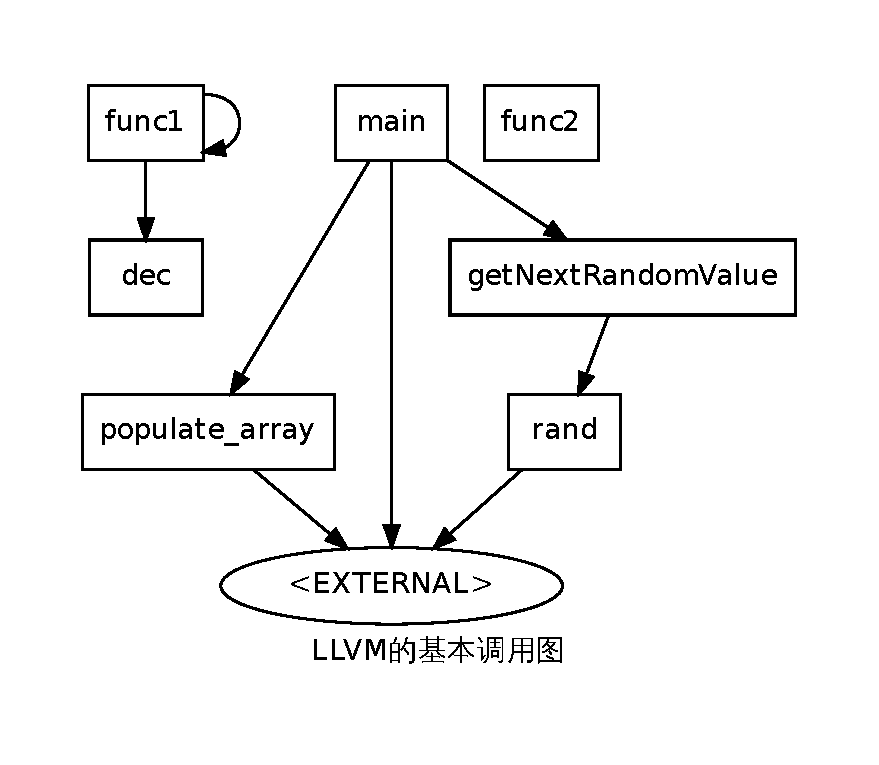
\includegraphics[width=.6\textwidth]{fig/cg_llvm.pdf}}
\hspace{1in}
\subfigure[Accurate Call Graph]{\label{fig:accurate_cg}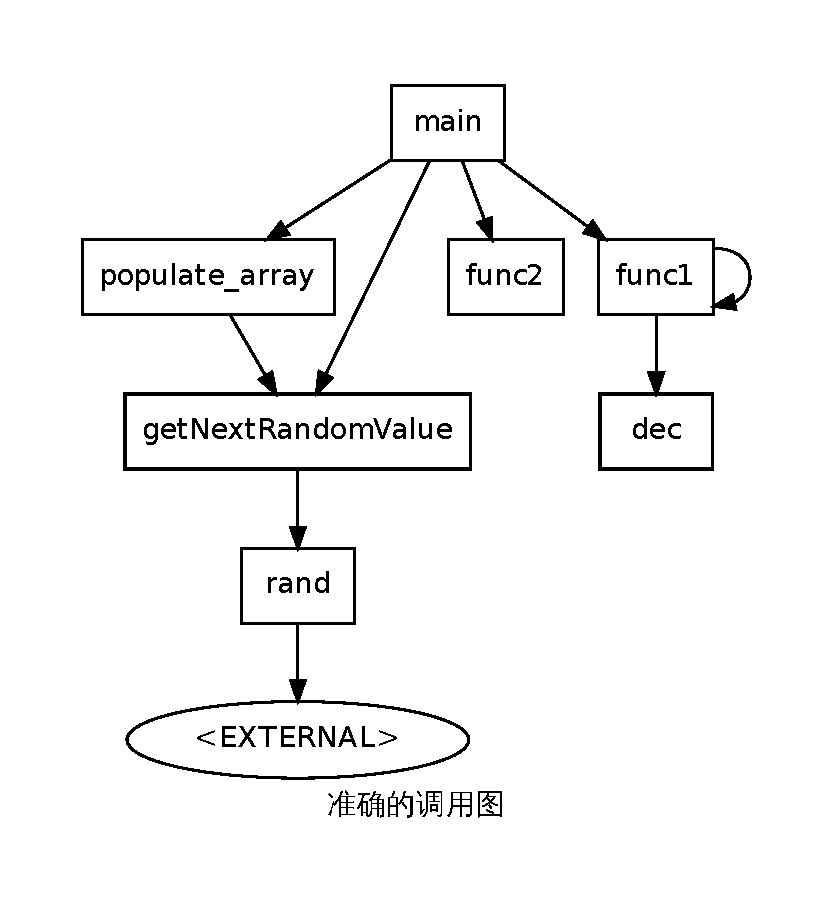
\includegraphics[width=.6\textwidth]{fig/cg.pdf}}
\bicaption[fig:callgraphs]{调用图比较}{调用图比较}{Fig}{Comparison of Call Graphs}
\end{figure*}

经过该算法得到的调用图仍然会存在外部节点,这是因为部分函数没有定义而只有声明,无法判断其调用信息。对于一个可执行程序,这样的函数来自于:
\begin{enumerate}[label={(\arabic*)}]
\item 外部库函数
\item 未使用的函数声明(例如头文件的函数声明)
\end{enumerate}
若为情形(1),可以保证该库函数不会调用任何一个在该编译单元中的函数;对于情形(2),这类函数可通过\autoref{sec:uncalled}中的方法消除。

\section{基于未被调用函数的削减}
\label{sec:uncalled}

对已建立的函数调用图,给定程序的入口函数(如main函数)仍可做一些额外的削减。这是因为在同一个编译单元里的函数有可能不会被调用(即在调用图上,从入口函数到该函数之间没有路径)。步骤如下:
\begin{algorithm}\label{alg:uncalled}
\caption{未被调用函数的削减}
\SetAlgoNoLine
遍历编译单元中的函数表,若该函数不在Caller2CalleeMapentry中,将该函数的函数体置空,并标记为待删除函数。

遍历待删除函数集合,逐一从编译单元中删除。
\end{algorithm}

该过程同时解决了\autoref{subsec:cg_impl}中的外部节点的情形(2)所带来的外部节点问题。本操作的必要性将在\autoref{sec:inter-reach}提及。

\section{基于可达性的削减}
\label{sec:reach}

\subsection{过程内分析}
\label{subsec:intra-reach}

过程内的可达性分析将函数调用点看作普通节点。LLVM的中间表示形式中的每个函数以基本块划分为不同的节点,且可以保证单一的入口;同时可以通过PHI函数合并使得仅有一个return语句。考虑函数中任意基本块是否可以执行到某一特定基本块(语句或指令层的可达性可以由基本块迅速导出),该问题退化为一般的图可达性问题,通过经典的DFS/BFS算法实现。\autoref{sec:inter-reach} 的分析说明不能将过程内的不可达分析用于削减。

\subsection{过程间可达性}
\label{sec:inter-reach}

由于所关注的语句所在函数可能被调用多次,在同一函数内对同一条语句(或指令)过程内可达集合是过程间可达的子集。以下述程序为例说明其差异性。

\begin{figure}[t]
\begin{center}
\begin{lstlisting}[language={[ANSI]C}]
int foo(int i) {
  if (i < 0) {   
/// interest point
    return -i;
  } else {
    return i;
  }
}

int foo1(int i) { return foo(i); }

int foo2(int i) { return foo(i); }

int main(void) {
  int i = -1;
  foo2(-i);
  foo(i);
  return 0;
}
\end{lstlisting}
\bicaption[fig:reach]{可达性分析典型例子}{可达性分析典型例子}{Fig}{A Classic Example about Program Reachability}
\end{center}
\end{figure}
以foo函数中的if分支的return语句作为关注点,在分析过程内可达性时,else分支不可以通过任何路径达到该点。然而在过程间分析时,由于foo2调用了foo之后foo又被main函数直接调用,静态分析需保守认为存在一条在foo2调用foo时执行了else分支、而foo执行了if分支,故在过程间分析中else分支的语句需被计入可达关注点的集合中。 另一方面,foo1中的调用函数foo的语句可以达到关注点,然而因为foo1没有被入口函数调用(这里为main),故不可达关注点,这正是\autoref{sec:uncalled}削减未调用函数的原因。

不同于过程内的可达性分析,过程间的分析必须关注函数调用点——在函数调用前后的可达性是截然不同的。这需要我们特殊对待基本块中的调用点前后。其实现参见算法\ref{alg:reach}。

\begin{algorithm}\label{alg:reach}
\caption{可达性算法}
\SetAlgoNoLine

将每个基本块以函数调用点为界限划分为多个“子基本块”。初始认为仅关注点所在子基本块可达。

(1)在过程内计算可达性,更新该子基本块为可达。(2)将可达调用点的所有未完全被访问(函数中至少存在一个调用点未被访问)的被调函数及该被调函数的所有未完全被访问的callee(Caller2CalleeMap)的所有基本块都更新为可达,标记所有的callee的所有调用点为已访问。

根据directCallee2CSMap得到关注点所在函数的所有未被访问的被调用点(采用队列的方式)。
将每个被调用点作为间接关注点,标记重复step2,step3中的操作直至(1)所有函数中的调用点都被访问过。
\end{algorithm}

需要注意的是,这里不考虑特殊的函数调用会影响可达性结果:例如exit()函数调用处于某个基本块中间;或setjmp/longjmp函数调用等。

\subsection{基于可达性的削减}
\label{subsec:reach-prune}

并非所有的不可达语句均可削减,这是因为不适当的削减会导致程序不可执行,而错误的基本块拼接会影响到关注点的执行路径。实现时将这些分支的内容转换成立即退出的特殊函数调用:
\begin{algorithm}\label{alg:reach-prune}
\caption{基于可达性的削减}
\SetAlgoNoLine
对编译单元中的每一个基本块(或子基本块)计算其到关注点的可达性,将不可达节点放入不可达集合中,并将不可达节点所在的终结指令替换成LLVM中的不可达指令。

遍历不可达集合中的基本块(或子基本块中所在基本块):若未被用,则将该块内容置空,并将该块从编译单元中删除;若其仍被使用,则将该块内容替换成exit(1)的函数调用。
\end{algorithm}


\section{基于程序影响性分析的削减}
\label{sec:slicing}

程序切片比基于可达性的削减更为精确,后者的削减结果是仅包含实际可执行至关注点的语句,而前者进一步剔除那些可达到关注点、但并不影响关注点结果的语句。类似于可达性分析,程序切片过程间的分析集合比过程内的分析更为保守安全;与可达性分析不同,这里的分析完全应用于LLVM的指令层次。过程间分析采用了Mark Weiser提出的基于控制流图的过程内分析和过程间调用点传递的方式~\upcite{Slicing81}。
% \todo{add algo}

细节上有如下改变:
\begin{enumerate}
\item 由于部分LLVM的IR中的指令的结果值本身为变量(如LoadInst/CastInst或返回值的CallInst等),在实现过程中不严格区分语句和变量而只关心指令和其操作数。对每一读写内存操作,考虑其可能的指针变量的指向集合,并在函数的调用处分析其修改变量信息。
\item 经典切片算法中不涉及程序Load/Store这类内存相关指令,为此首先使用了LLVM的mem2reg这一转换,消除了程序中不必要的内存读写指令。同时将Store操作的指令所写地址既作为定义(DEF)又作为使用(REF),这是因为LLVM既对所写地址变量直接操作(类似于地址运算),又可以对地址处的内容所存放值运算(通过Load)。对其他切片算法中没有的指令类型,采用类似的手段进行模拟。
\item LLVM的IR要求每个基本块必须以终结指令结束,故必须保留分支跳转语句、switch语句等。然而存在跳转的条件变量为undef的削减结果,这对应该分支为不相关分支的情形,可以通过LLVM的PHI函数解决。
\end{enumerate}
这是一个不动点的算法,每一次相关集的改变都需要重新修改甚至整个编译单元的相关集,代价是巨大的。将\autoref{sec:reach}中的过程间可达性算法与之结合,可以在实际中大大削减分析开销。

经过程序切片得到的\rbscope 是仅由程序可达性分析得到的\rbscope 的一个精化。直观而言,它包含的语句在执行时可能生成的路径需满足:
\begin{itemize}
\item 连接了\prog\ps 和\prog\bs
\item 对程序中的断言\prog\ass 上的条件值有影响
\end{itemize}

这里没有使用forward slicing用来计算\prog\ps 影响到的程序片段,其原因参见\autoref{chap:fwd_issue}。

\section{本章小结}
\label{sec:c3}

本章具体阐述了\rbscope 的生成算法。首先给出了\rbscope 的生成流程图,对其依赖关系作了解释。接着,对\rbscope 生成中的每个步骤进行了详尽的说明,分别是\nameref{sec:config}、\nameref{sec:andersen}、\nameref{sec:callgraph}、\nameref{sec:uncalled}、\nameref{sec:reach}、\nameref{sec:slicing},对于没有经典实现的分析或转化算法给出了其在LLVM中间代码上的具体实现。